\documentclass[onecolumn,12pt,tightenlines, a4paper,superscriptaddress,notitlepage]{revtex4-1}
\usepackage[utf8]{inputenc}
\usepackage{amsmath}
\usepackage{amsfonts}
\usepackage{amssymb}
\usepackage{graphicx}
\usepackage{kpfonts}
\usepackage{siunitx}
\usepackage{hyperref}

\usepackage{pgfplots}
\usepackage{pgfplotstable}
\pgfplotsset{compat=1.9}

%\definecolor{Main}{rgb}{0.74, 0.13, 0.19}
\definecolor{Accent1}{rgb}{0.5,0.5,0.5}%{0.76,0.36,0.13}
%\definecolor{Accent2}{rgb}{0.54,0.1,0.4}



\begin{document}

\title{Yoghurt under stress}
%\date{}

\author{\bf Mathieu Leocmach}
\email{mathieu.leocmach@univ-lyon1.fr}
\affiliation{Institut Lumière Matière, Lyon}
\author{C.~Perge}
\affiliation{Laboratoire de Physique, ENS de Lyon}
\author{T.~Divoux}
%\email{divoux@crpp-bordeaux.cnrs.fr}
\affiliation{CRPP, Bordeaux, France}
\author{S.~Manneville}
\affiliation{Laboratoire de Physique, ENS de Lyon}

\maketitle

Mouthfeel is a complex, multidimensional  sensory experience, whose design is critical to the success of a dish or a food product. Here we investigate the mechanical behaviour of a model yoghurt under large deformation. Biomaterials such as protein or polysaccharide gels are known to behave qualitatively as soft solids and to rupture under an external load. Combining optical and ultrasonic imaging to shear rheology we show [\href{http://link.aps.org/doi/10.1103/PhysRevLett.113.038303}{Leocmach et al., Phys. Rev. Lett., 2014, 113, 038303}] that the failure scenario of an acid-induced sodium caseinate gel is reminiscent of brittle solids: after a primary creep regime characterized by a power-law behavior whose exponent is fully accounted for by linear viscoelasticity, fractures nucleate and grow logarithmically perpendicularly to shear, up to the sudden rupture of the gel. A single equation accounting for those two successive processes nicely captures the full rheological response. The failure time follows a decreasing power law with the applied shear stress, similar to the Basquin law of fatigue for solids. These results are in excellent agreement with recent fibre-bundle models that include damage accumulation on elastic fibres and exemplify protein gels as model, brittlelike soft solids.

\vfill
\begin{center}
%\begin{figure}
\let\mylena\relax
\newlength\mylena
\pgfmathsetlength{\mylena}{0.19\textwidth}
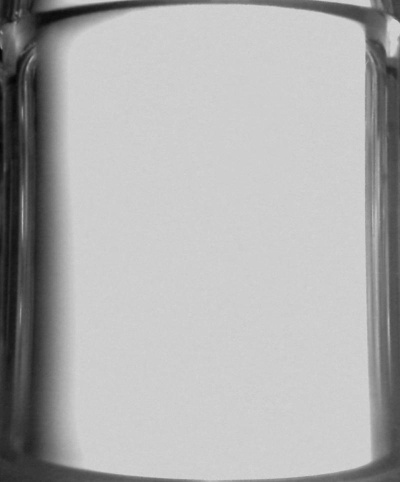
\includegraphics[width=\mylena]{Y110_2013-03-01_02-55-11.jpg}\hfill
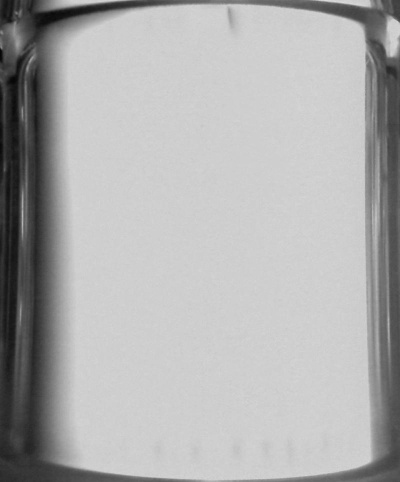
\includegraphics[width=\mylena]{Y110_2013-03-01_03-06-28.jpg}\hfill
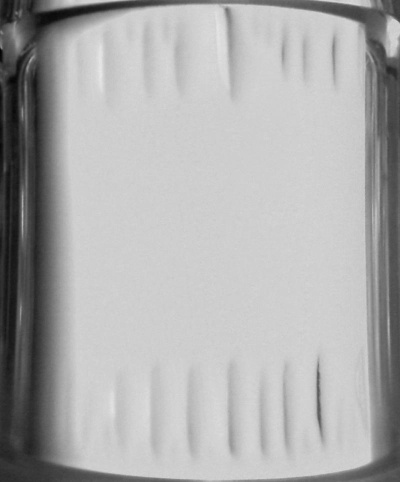
\includegraphics[width=\mylena]{Y110_2013-03-01_03-19-47.jpg}\hfill
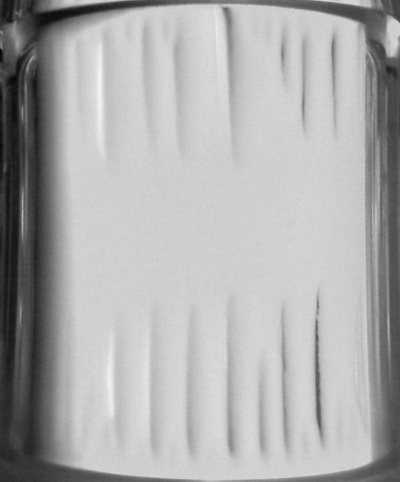
\includegraphics[width=\mylena]{Y110_2013-03-01_03-21-10.jpg}\hfill
%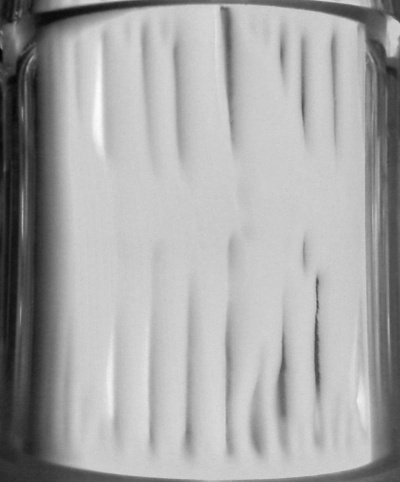
\includegraphics[width=\mylena]{Y110_2013-03-01_03-21-18.jpg}\hfill
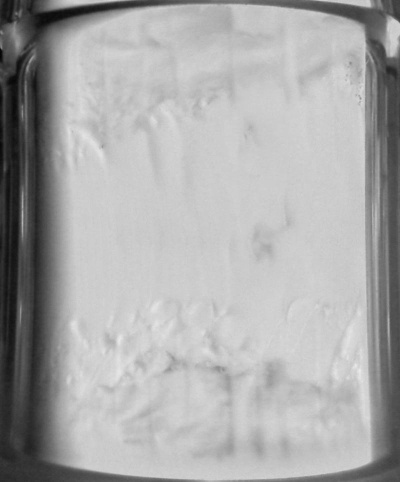
\includegraphics[width=\mylena]{Y110_2013-03-01_03-21-19.jpg}\\

\vspace{0.2em}
\hfill\begin{tikzpicture}
\begin{axis}[
	width=0.975\textwidth,
	height=12\baselineskip,
	xmode=log,
	ymode=log,
	xlabel={$t$ (\si{\second})},
	xmin=0.1,
	ylabel={strain rate $\dot\gamma$ (\si{\per\second})}, 
	ymin=0.9e-4, ymax=2e-1,
	axis on top,
	]
 	\fill[Accent1!20]
		(axis cs:3,1e-2) ellipse[rotate=-17.5, x radius=0.4\textwidth, y radius=0.04\textwidth] node[below, rotate=-17.5, black] {power-law creep}
		(axis cs:0.8e3,2e-4) ellipse[x radius=0.05\textwidth, y radius=0.02\textwidth] node[below, black] {nucleation}
		(axis cs:1577,1e-2) ellipse[x radius=0.04\textwidth, y radius=4\baselineskip] node[below, rotate=90, black] {explosive regime}
		;
	\addplot[thick] table {Y110_300Pa.gdot}; 
	\addplot[thick, only marks, mark=o] coordinates {(687, 2.1e-4) (1476, 7.35e-4) (1509, 1.12e-3)};
	\node[below] at (rel axis cs:0.5,1) {Couette cell $\sigma=\SI{300}{\pascal}$};
\end{axis}
\end{tikzpicture}%
%\caption{Optical visualisation of fractures in a casein gel confined between two concentric cylinders submitted to a constant shear stress (right) with the corresponding local strain field (in \si{\micro\metre}) measured by ultrasound echography in a vertical slice. Scale bars are in millimetres.}
%\end{figure}
\end{center}


%We investigate the robustness of this scenario with varying acidulent concentrations, paying special attention to the case of over-acidified gels previously overlooked in the literature. Qualitative differences are explained by microstructural changes below isoelectri pH that we monitor throughout gelation both by rheology and confocal microscopy. As a whole, our results highlight protein gels as a versatile and model system for the study of plasticity in soft amorphous materials.
\end{document}